\subsection{MF Letters $n$-grams}

Instead of considering every token as a word, another popular method is to create a "word" from a short sequences of letters called letters $n$-grams using Definition~\ref{def:letters_n_grams}.
To consider overlapping words, the whole document is synthesized into a long string by joining every token by an \textit{underscore} : $\_$, to remove visual ambiguity due to the nature of the space character.
This technique can be further explored by combining for example two or more $n$-grams sizes together.
$n$-grams can be really effective even though no clear meaning from each $n$-grams can be exploited at first sight.
A simple explanation on why $n$-grams can be effective is by using $n$-grams of size 3 to 5 in most Germanic languages this can correspond to for example : the tense of the verbs (i.e. : \textit{"ing\_"}, \textit{"ed\_"}), some small common words (\textit{"\_the\_"}, \textit{"\_and\_"}, \textit{"\_that"}), or in French the adverbs (\textit{"\_ment"}) which can capture the style of an author.

\begin{definition}[Letters $n$-grams]
  \label{def:letters_n_grams}
  A letter $n$-grams is a tokenization which is constructed by creating a token of size $n$ for each substrings starting from the position $0$ to \textit{text\_size} $- n - 1$.

  Example: \\
  Using 3-grams the string: \textit{"fox\_is\_brown"} \\
  is converted to: (\textit{"fox", "ox\_", "x\_i", "\_is", "is\_", "s\_b", "\_br", "bro", "row", "own"})
\end{definition}

An alternative version of the $n$-grams algorithm used here is defined in Definition~\ref{def:words_n_grams}.
This algorithm considers each token as a string to apply the letters $n$-grams algorithm to.
To differentiate it from the classical $n$-grams algorithm.
The latter algorithm, is called in this study In-word $n$-grams (Definition~\ref{def:words_n_grams}) and the other one is called letters $n$-grams (Definition~\ref{def:letters_n_grams}).

\begin{definition}[In-words $n$-grams]
  \label{def:words_n_grams}
  In-word $n$-grams are created by applying the letters $n$-grams algorithm on each token.
  When a token is smaller than $n$, the whole token is considered.

  Example: \\
  Using words 3-grams on the following tokens: ["fox", "is", "brown"] \\
  is converted to: (\textit{"fox", "is", "bro", "row, "own"})
\end{definition}

\subsubsection{Evaluation}

In this experiment the whole text is considered to create letters $n$-grams for the text representation, see Definition~\ref{def:letters_n_grams}.
As for the other experiment, the MFW approach is used to create the feature vector.
To reduce the field of the possible parameters, the experiment is split in two parts :
The first part is to find the size of the $n$ parameter of the $n$-grams, and the number of MFW.
The second is to compare the distance metrics with the previously found parameters.

One of the main drawback with this approach is that some distance metrics can have better performance on highly dimensional vectors (large MFW vector) than others, and thus this methodology does not take into account this.

\subsubsection{Evaluation first part}
For the first part, the Z-Score normalized cosine distance measure is used to compare the vectors and create the rank list.
The parameters used are: a varying MFW vector size ranging between 500 and 15000 with a step of 500 and an $n$ for the following values : $3, 4, 5, (2, 3), (3, 4), (4, 5)$.
The tuples $(a, b)$ correspond to both $a$-grams and $b$-grams in the same text representation.

The number of different $n$-grams is assumed to be larger than the vocabulary of the texts, thus the importance of having a larger vector when dealing with long texts such as the literature datasets.
When considering letters $n$-grams the text representation increases approximately by a factor of $t$, with $t$ being the average token length.
The average token size for the literature dataset is displayed Table~\ref{tab:lit_corpora} in Chapter~\ref{sec:definitions_and_corpora}, and is around $4$ characters.
To avoid having too large text representation, a possible idea is to remove the hapax legomena (tokens appearing only once in the corpus) before applying the $n$-grams algorithm.
This method can also be generalized to remove words appearing less than $x$ times.
This pruning approach was explored in~\cite{kocher_linking} but was not used in this study.

Figure~\ref{fig:letter_ngrams} show the results of the first part of the experiment on the Oxquarry dataset (\ref{fig:letter_ngrams_oxquarry}), Brunet (\ref{fig:letter_ngrams_brunet}) and St-Jean (\ref{fig:letter_ngrams_st_jean}).
The trends seem to indicate that a lower $n$ value converge with lower MFW vector size but reach a maximal value faster.
With $3$-grams, $\sim 3000-4000$-MFW give good results on both datasets with this distance metric.
On the Brunet dataset, after reaching the maximal average precision at $\sim 4000$-MFW, a larger number of frequent words decrease the precision until reaching the maximal number of different $3$-grams at $\sim 6500$-MFW, which is not the case on Oxquarry.
On St-Jean, the $3$-grams and $(2,3)$-grams do not reach a high average precision with a low number of MFW like for the Brunet and Oxquarry.
$4$-grams also can be efficient but require a larger MFW vector, around $\sim 4000$-MFW give good result for both Brunet and St-Jean but on Oxquarry it requires around $\sim 8000$ to have similar results as the $3000$ $3$-grams.
For the first part, the retained parameters for the $n$-grams text representation are the $3$-grams with $3000$-MFW and $4$-grams with $8000$-MFW.

\begin{figure}
  \caption{Letters $n$-grams representation over number of MFW with different $n$}
  \label{fig:letter_ngrams}

  \subcaption{Oxquarry}
  \label{fig:letter_ngrams_oxquarry}
  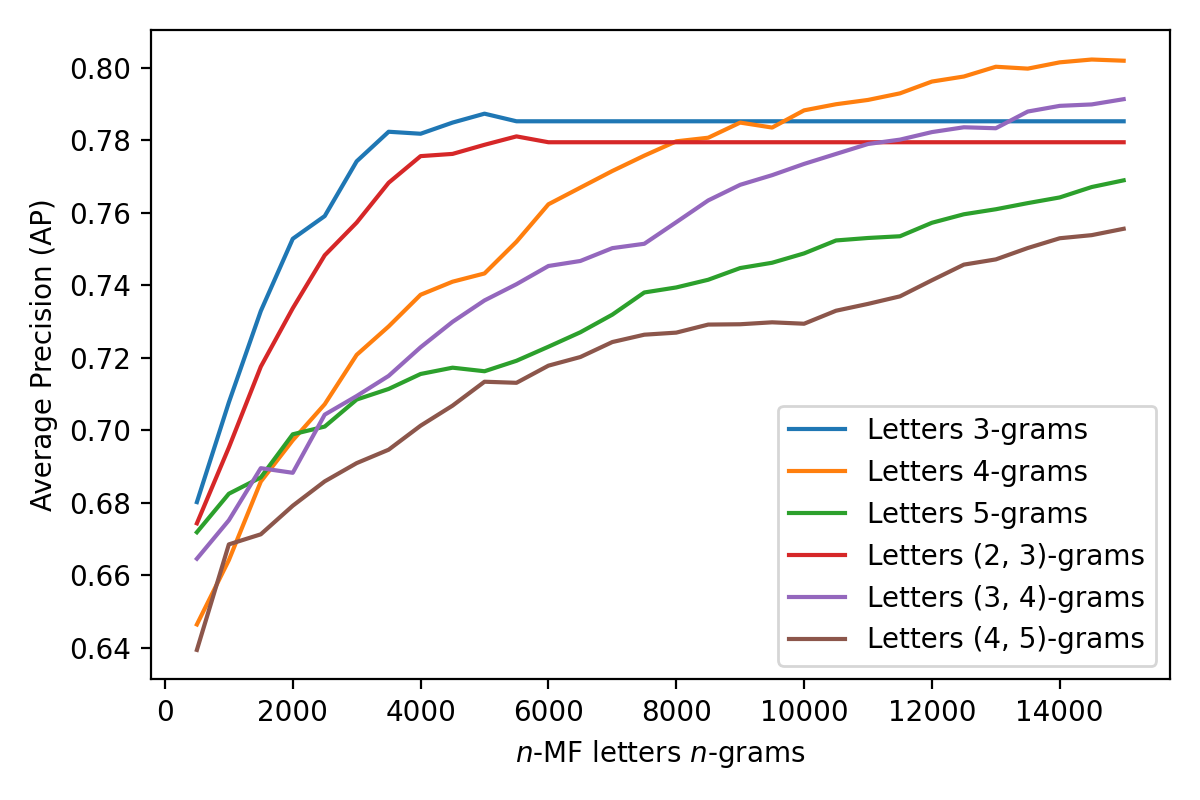
\includegraphics[width=\linewidth]{img/letter_ngrams_oxquarry.png}

  \vspace{0.5cm}

  \subcaption{Brunet}
  \label{fig:letter_ngrams_brunet}
  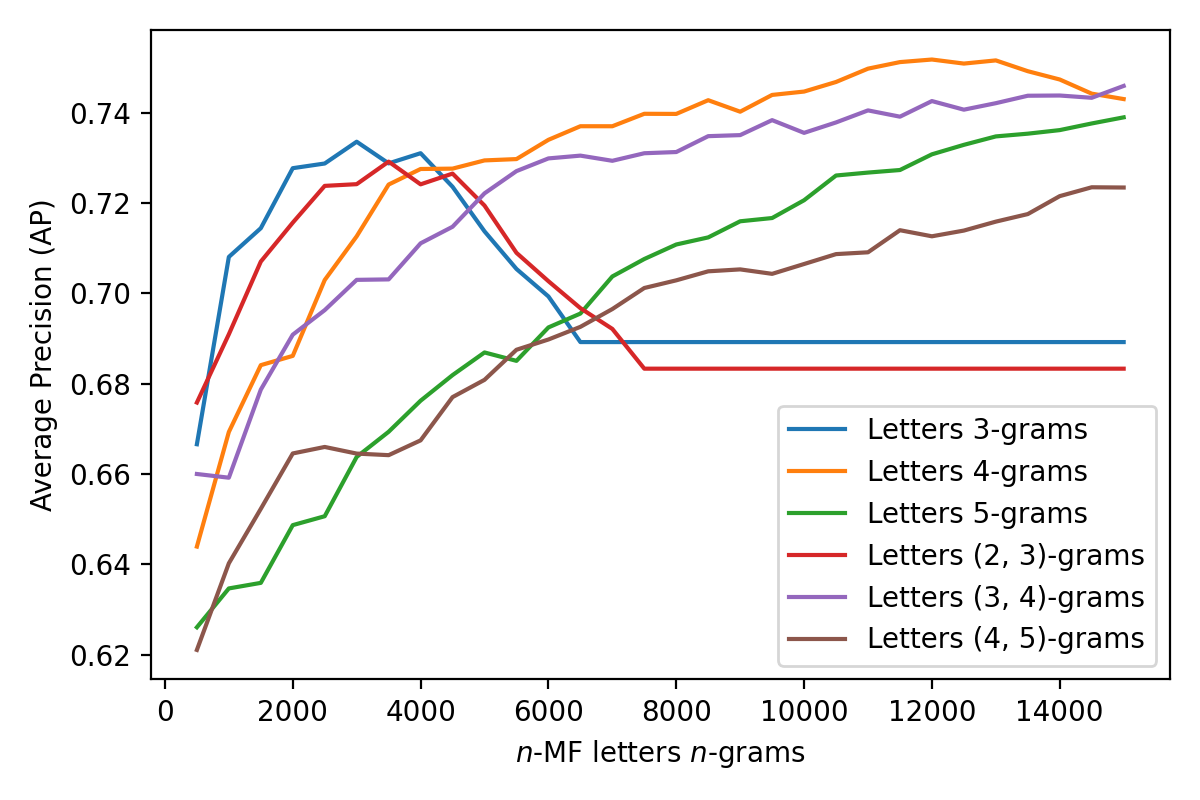
\includegraphics[width=\linewidth]{img/letter_ngrams_brunet.png}

  \vspace{0.5cm}

  \subcaption{St-Jean}
  \label{fig:letter_ngrams_st_jean}
  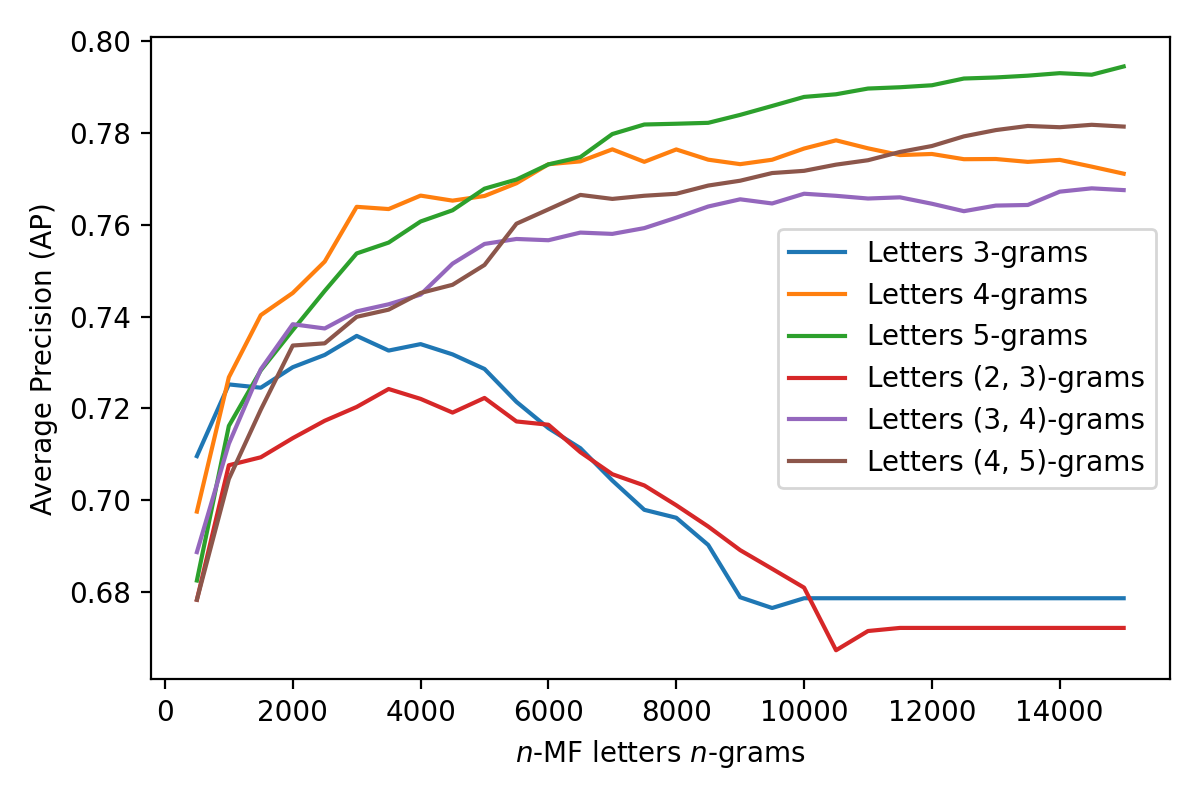
\includegraphics[width=\linewidth]{img/letter_ngrams_st_jean.png}
\end{figure}

\subsubsection{Evaluation second part}

As stated earlier, in the second part the objective it to compare the distance metrics with the $3$-grams/$3000$-MFW and $4$-grams/$8000$-MFW.
The distance metrics used are the ones presented in Section~\ref{sec:vectors_distances}.
The results for this experiment are in Table~\ref{tab:letter_ngrams}.
Since the number of MFW and the size of the $n$-grams was optimized on the Cosine distance, the results may be biased.

For the $3$-grams, the following results can be observed:
The Cosine distance give the best results.
Though, two distances metrics can compete with the Cosine distance on certain datasets with the $3$-grams approach, namely the Manhattan distance and the Clark distance.
A worth noticing results, is the Euclidean distance, which have polarized results: on Oxquarry the average precision is $0.72$ and on St-Jean only $0.47$.
Using the right distance measure can have a relative increase up to $36$\%, when comparing the worse distance metric to the best of each dataset.

For the $4$-grams approach, as for the $3$-grams the Cosine is the best measure with this configuration.
The Manhattan distance and the Clark distance also are the second choice.
The Euclidean distance have the same behaviour as for $3$-grams on the dataset.
For this configuration of $4$-grams with $8000$-MFW, using the right distance measure is less impactful than the $3$-grams approach but still can have a relative increase in performance of $28$\% when changing from the worse distance metric to the best, with these datasets.

\begin{table}
  \centering
  \caption{Average precision for $n$-grams with every metrics, on the 3 datasets (best result for the dataset in bold).}
  \label{tab:letter_ngrams}

  \subcaption{$3$-grams with $3000$-MFW}
  \begin{tabular}{l c c c}
    \toprule
    Distance metric & Oxquarry & Brunet & St-Jean \\
    \midrule
    Manhattan & \textbf{0.77} & 0.66 & 0.62 \\
    Tanimoto & 0.64 & 0.66 & 0.62 \\
    Euclidean & 0.72 & 0.63 & 0.47 \\
    Matusita & 0.60 & 0.66 & 0.58 \\
    Clark & 0.64 & \textbf{0.73} & 0.63 \\
    Cosine & \textbf{0.77} & \textbf{0.73} & \textbf{0.74} \\
    KLD & 0.57 & 0.65 & 0.54 \\
    JD & 0.58 & 0.66 & 0.56 \\
    \bottomrule
  \end{tabular}

  \vspace{0.5cm}

  \subcaption{$4$-grams with $8000$-MFW}
  \begin{tabular}{l c c c}
    \toprule
    Distance metric & Oxquarry & Brunet & St-Jean \\
    \midrule
    Manhattan & 0.76 & 0.69 & 0.73 \\
    Tanimoto & 0.68 & 0.68 & 0.68 \\
    Euclidean & 0.73 & 0.65 & 0.55 \\
    Matusita & 0.63 & 0.68 & 0.65 \\
    Clark & 0.67 & 0.72 & 0.75 \\
    Cosine & \textbf{0.78} & \textbf{0.74} & \textbf{0.78} \\
    KLD & 0.61 & 0.66 & 0.60 \\
    JD & 0.61 & 0.67 & 0.63 \\
    \bottomrule
  \end{tabular}
\end{table}

\subsubsection{MFW First letters, last letters, word $n$-grams of tokens}

In this experiment, the goal is to create 3 types of text representations of word substrings and compare them.

\begin{enumerate}
  \item
  The first representation is the $n$-first letter of each word tokens which correspond generally to the meaning of a word.
  If the word token is smaller than N, the whole word is used.
  \item
  Extract also the $n$-last letter of each word tokens, which in this case correspond to the role of the word in a sentence.
  As for the previous representation, if the word is smaller than N, the whole word is used instead.
  \item
  The in-word $n$-grams (See Definition~\ref{def:words_n_grams}), this special type of n-grams consider only $n$-grams within a word.
  This excludes every overlapping word when considering the Letters $n$-grams algorithm.
  This decision is made for this experiment such that inter-words informations can not be learned and have a fair comparison of these 3 texts representations.
\end{enumerate}

The first approach can be related to the lemma approach, the second to the POS approach and the third to a hybrid version between the letters $n$-grams and the word token text representations.
The two first representations have the same number of words as the token text representation and are a subsets of the third method.
The third representation is a subset of the Letters $n$-grams text representation.

For this experiment the only distance measure used is the Z-Score normalized Cosine distance and, for the evaluation metric, only the average precision.
The number of MFW variate for this experiment between 200 and 4000 with a step of 100.
Figure~\ref{fig:first_last_letters_ngrams} shows the results for this experiment on the three datasets (Oxquarry, Brunet, St-Jean).

In the three dataset, the 3-last letters and 3-first letters gives a lower average precision and quickly converge to an equilibrium value at around 1500 MFW.
5-letters representations tend to produce better results than 3-letters and 4-letters representation as the MFW increase.
In the Oxquarry corpus, in-word $4$-grams and in-word $5$-grams give an outstanding ~95.0\% in average precision, but is not as efficient for the Brunet dataset.
For the Brunet dataset, the 5-first letters can a good results compared to other text representations with small MFW vector size.
And for St-Jean, the 5-first letters with a small MFW vector size giv the best results.
No clear best configuration can be extracted with these results since the results are mixed across datasets, thus for this experiment, no text representation / distance measure are retained for the fusion.

\begin{figure}
  \centering
  \caption{Average precision over the MFW in the rank list generated using the Z-Score normalized Cosine distance}
  \label{fig:first_last_letters_ngrams}

  \subcaption{Oxquarry}
  \label{fig:first_last_letters_ngrams_oxquarry}
  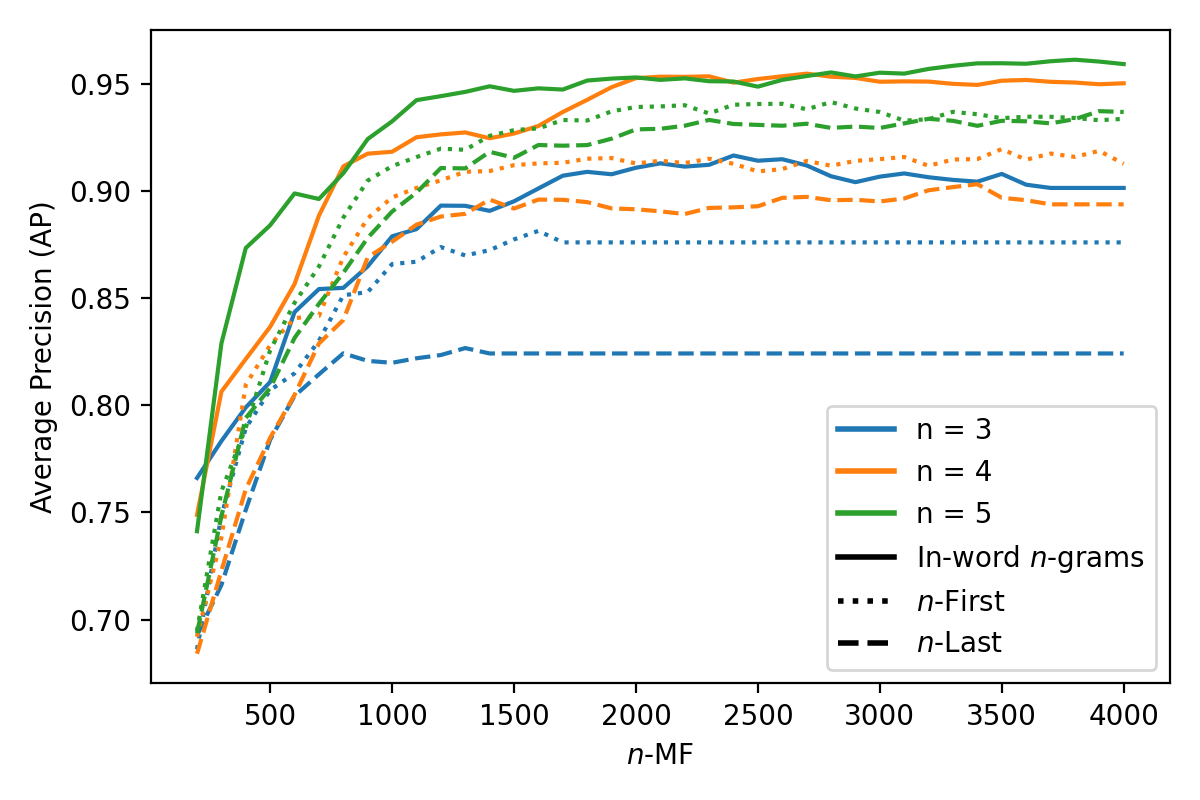
\includegraphics[width=\linewidth]{img/first_last_letters_ngrams_oxquarry.png}

  \vspace{0.5cm}

  \subcaption{Brunet}
  \label{fig:first_last_letters_ngrams_brunet}
  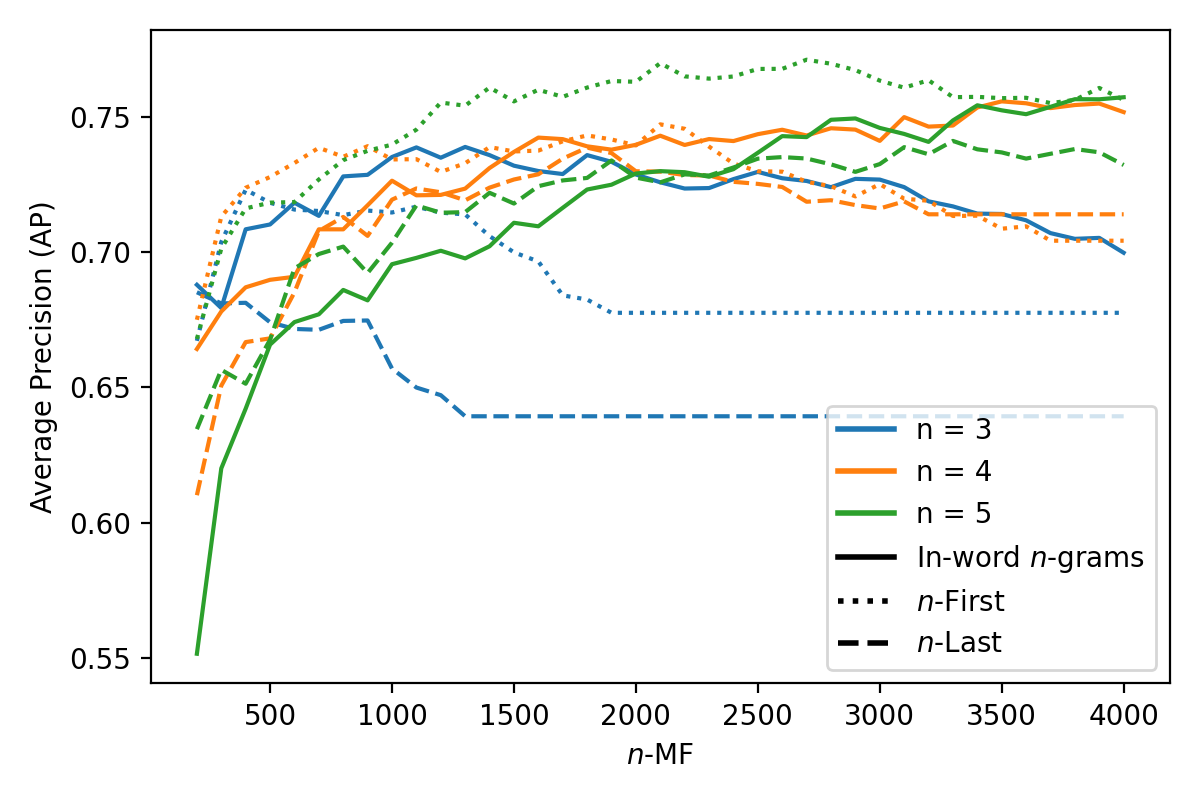
\includegraphics[width=\linewidth]{img/first_last_letters_ngrams_brunet.png}

  \vspace{0.5cm}

  \subcaption{St-Jean}
  \label{fig:first_last_letters_ngrams_st_jean}
  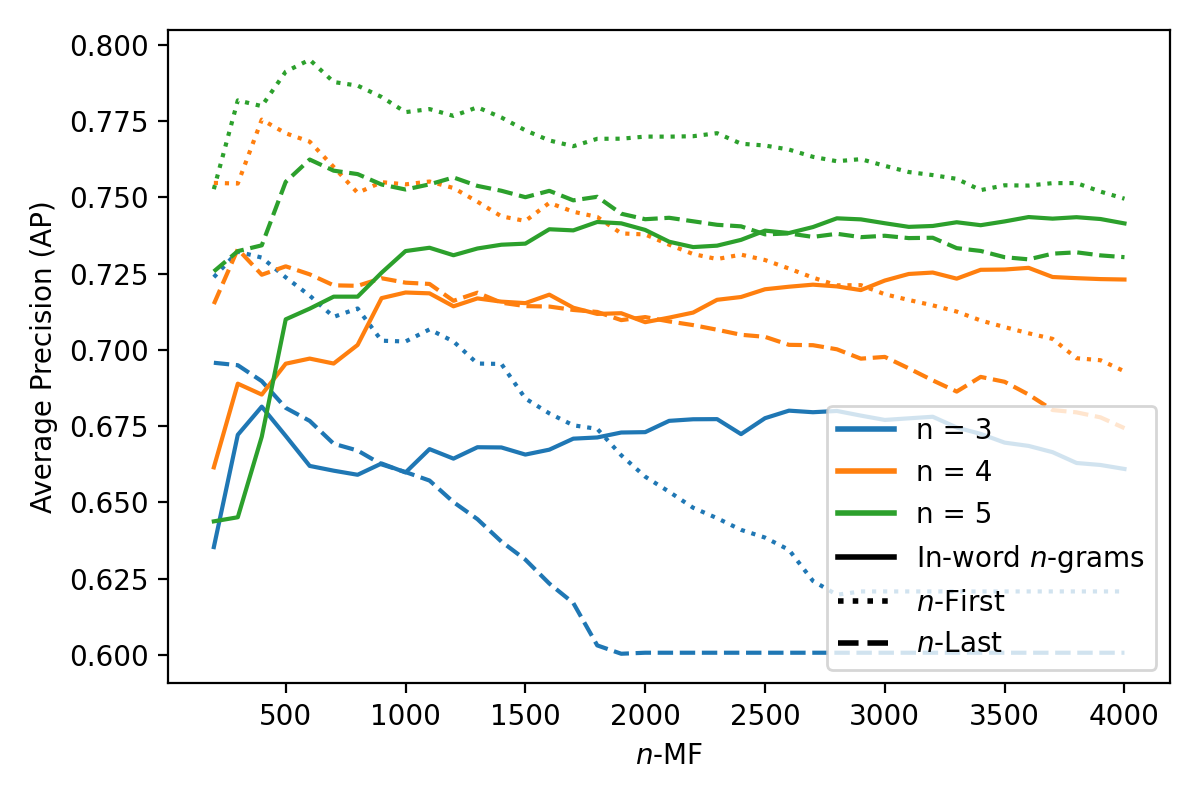
\includegraphics[width=\linewidth]{img/first_last_letters_ngrams_st_jean.png}
\end{figure}
